\section{Resultados}

\subsection{Implementação e simulação em Simulink}

A unidade de geração foi implementada em Simulink com solver de passo fixo (\texttt{ode4}) e passo de $T_s/100=0{,}5\ \mu$s, de modo que cada transição de chaveamento seja resolvida com precisão suficiente para a análise das ondulações. O modelo é organizado em quatro blocos: (i) a planta, que implementa as equações \eqref{eq:chav} com os estados $\mathbf{x}$ integrados; (ii) o bloco de PWM, no qual uma portadora dente-de-serra de frequência $f_s$ é comparada com as razões cíclicas, produzindo os sinais $s_b$, $s_c$ e $s_{pv}$; (iii) o controle, que reúne os PI de corrente \eqref{eq:pi}, o \textit{droop}, o filtro de demanda e as referências \eqref{eq:refs}; e (iv) os blocos de aquisição, que registram os estados e as razões cíclicas para o pós-processamento. A carga é uma fonte do tipo degrau, que reduz $R$ de 20~$\Omega$ para 16~$\Omega$ em $t=0{,}1$ s.

Sendo assim, três execuções foram realizadas a partir do mesmo modelo: a primeira com PWM e malha fechada, que fornece os sinais chaveados; a segunda com o modelo médio e malha fechada, em que as razões cíclicas atuam diretamente sobre as equações; e a terceira com razões cíclicas fixas e sem controle, utilizada como referência de comparação. Para os testes de equivalência, o circuito com as chaves $Q_1$ a $Q_6$ foi simulado com os mesmos comandos aplicados às equações, de acordo com a metodologia de três etapas.

\subsection{Verificação da equivalência por simulação em 3 etapas}

Em ambos os casos, a verificação comparou três etapas: o circuito chaveado (etapa 1), as equações chaveadas submetidas aos mesmos sinais PWM (etapa 2) e o modelo médio (etapa 3), este último comparado à média por período do circuito. Como as etapas 2 e 3 recebem apenas as razões cíclicas aplicadas, sem possuir malhas de controle próprias, eventuais diferenças em relação ao circuito decorrem da implementação das equações, das condições iniciais e dos métodos de integração, e não da ação do controlador. O primeiro período de chaveamento foi desconsiderado nas comparações envolvendo o modelo médio, pois a média móvel ainda está se formando.

\textbf{Sem controle.} As razões cíclicas calculadas, $d_b=0{,}5$, $d_c=0{,}25$ e $d_{pv}=0{,}375$, são mantidas constantes, a resistência de carga vale $20~\Omega$ e a simulação parte da condição inicial $\mathbf{x}(0)=(15~\mathrm{A},\,10~\mathrm{A},\,8~\mathrm{A},\,400~\mathrm{V},\,300~\mathrm{V})$. A janela de simulação é de $0{,}45$ s. Como não há regulação da tensão do barramento, $v_{dc}$ apresenta oscilações decorrentes da dinâmica dos indutores e do capacitor $C_{dc}$, enquanto as correntes dos indutores evoluem livremente, sem uma ação de controle que promova sua estabilização. A Figura~\ref{fig:equiv1} apresenta a comparação entre as etapas de simulação, enquanto a Figura~\ref{fig:scope1} apresenta os sinais originais registrados no \textit{Scope}.

\begin{figure}[H]
\centering
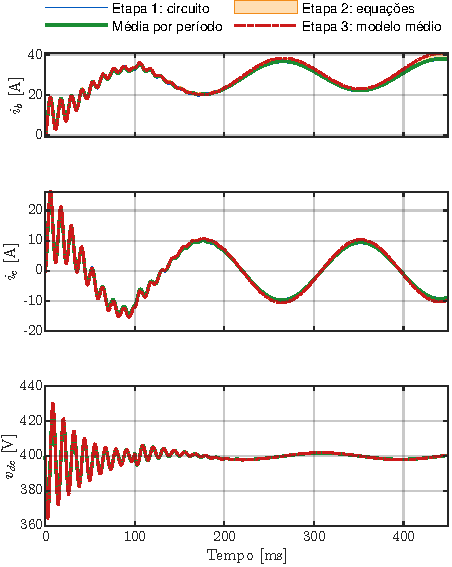
\includegraphics[width=\columnwidth]{images/fig_equiv1.pdf}
\caption{Sem controle: circuito (etapa 1), equações chaveadas (etapa 2), média por período e modelo médio (etapa 3) para $i_b$, $i_c$ e $v_{dc}$.}
\label{fig:equiv1}
\end{figure}

\begin{figure}[H]
\centering
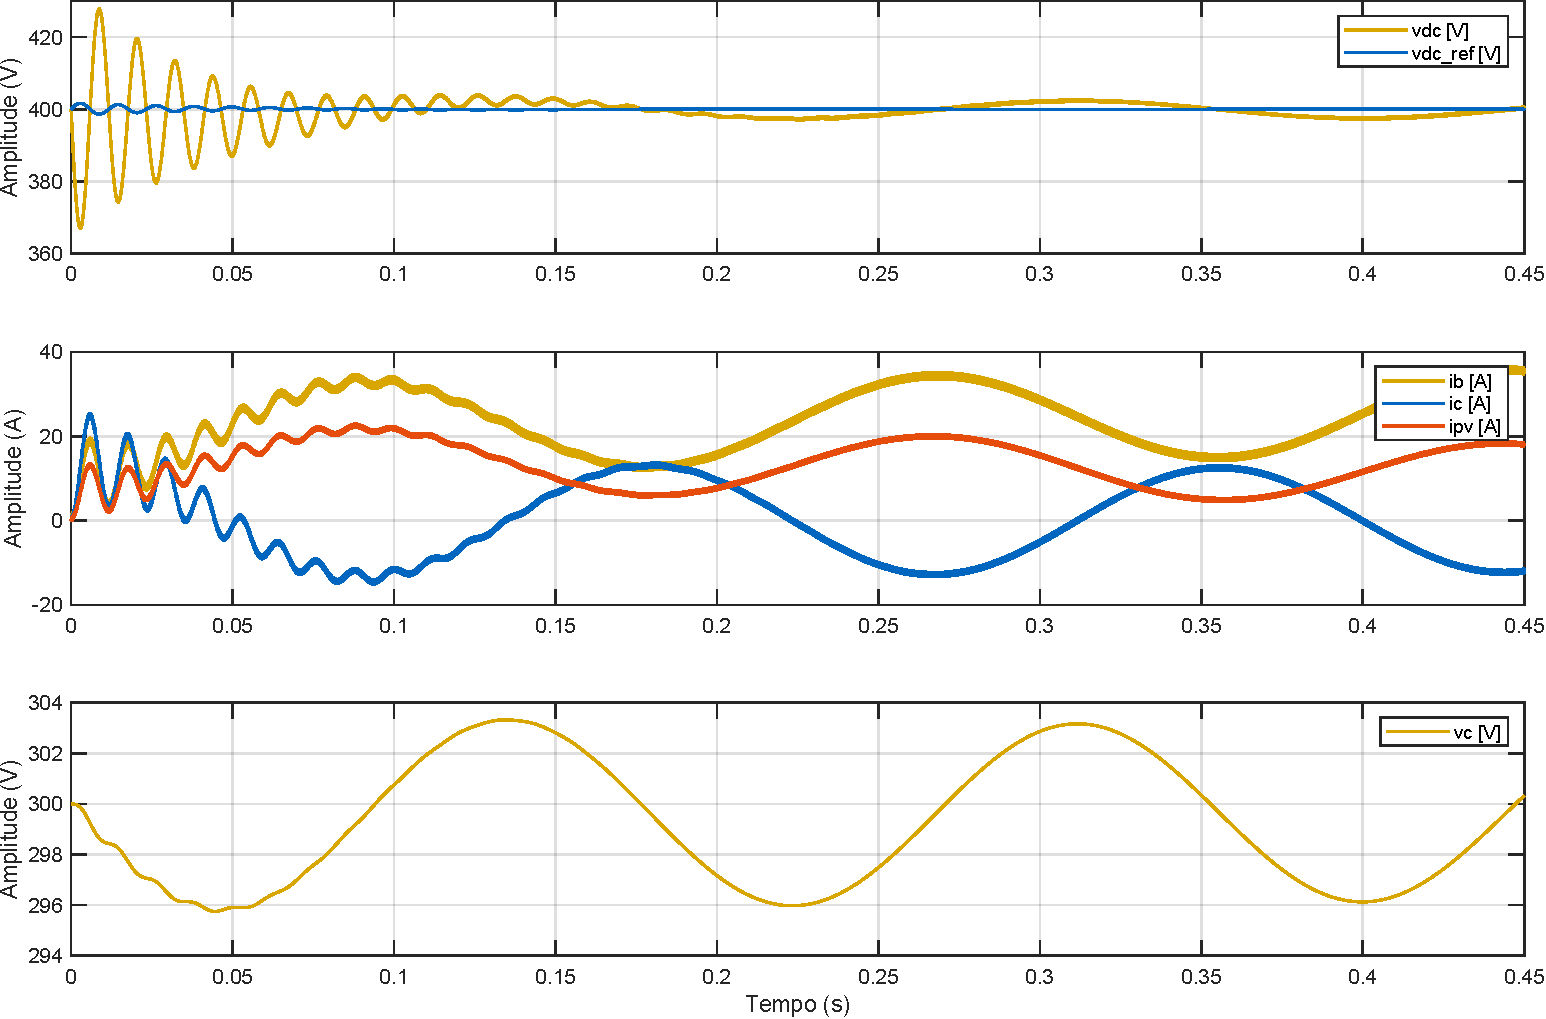
\includegraphics[width=\columnwidth]{images/Dados_semcontrole.pdf}
\caption{Sem controle: sinais do \textit{Scope} ($v_{dc}$, correntes dos indutores e $v_c$).}
\label{fig:scope1}
\end{figure}

 A simulação com controle parte do ponto de equilíbrio $\mathbf{x}(0)=(20~\mathrm{A},\,0~\mathrm{A},\,16~\mathrm{A},\,400~\mathrm{V},\,300~\mathrm{V})$ e, em $t=0{,}1$ s, a resistência de carga passa de $20~\Omega$ para $16~\Omega$. Nesse caso, o degrau provoca um aumento na corrente de carga, dada por $i_R=v_{dc}/R$, e, consequentemente, modifica a referência de tensão do barramento por meio da característica de \textit{droop}:

\begin{equation}
v_{dc}^{\star}=400-r_d(i_R-20),
\end{equation}

que passa de $400$ V para $V_f=395{,}294$ V. Assim, a ação do controlador modifica a dinâmica do sistema e a impedância de saída vista pela carga, ao passo que, no caso sem controle, as razões cíclicas permanecem fixas e não há uma referência de tensão a ser seguida. A Figura~\ref{fig:equiv2} apresenta a comparação entre as etapas de simulação, enquanto a Figura~\ref{fig:scope2} apresenta os sinais registrados no \textit{Scope}, incluindo a tensão do barramento e sua referência.

\begin{figure}[H]
\centering
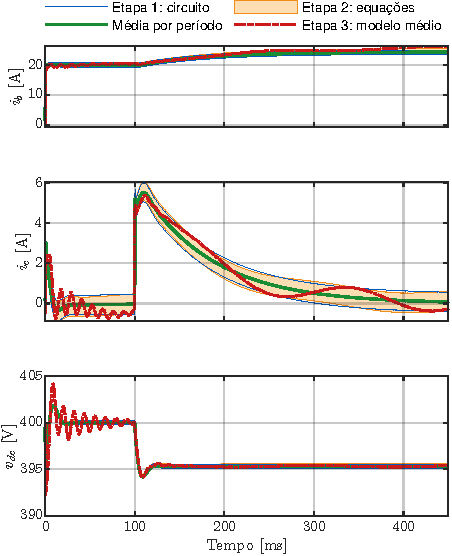
\includegraphics[width=\columnwidth]{images/fig_equiv.pdf}
\caption{Com controle: circuito (etapa 1), equações chaveadas (etapa 2), média por período e modelo médio (etapa 3) para $i_b$, $i_c$ e $v_{dc}$.}
\label{fig:equiv2}
\end{figure}

\begin{figure}[H]
\centering
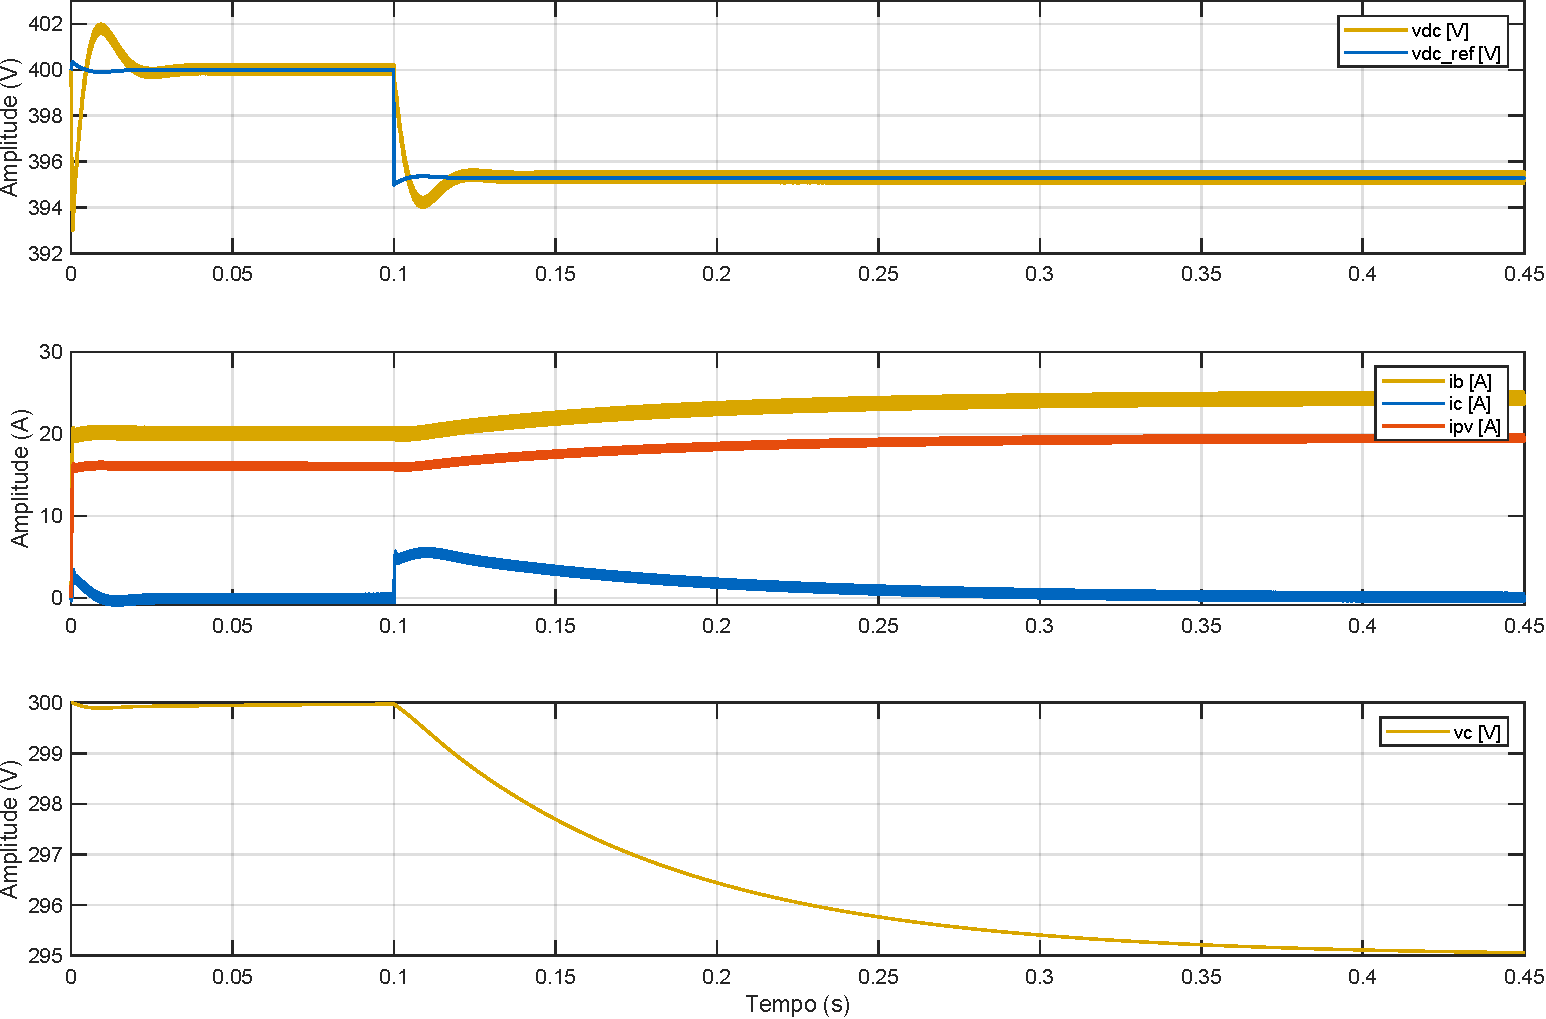
\includegraphics[width=\columnwidth]{Grafico_Conversor.pdf}
\caption{Com controle: sinais do \textit{Scope} ($v_{dc}$, $v_{dc}^{\star}$, correntes dos indutores e $v_c$).}
\label{fig:scope2}
\end{figure}

A Tabela~\ref{tab:erros} quantifica as diferenças entre as etapas 1 e 2 nos dois casos, por meio do erro máximo absoluto e do erro quadrático médio (RMS). A proximidade entre as curvas dessas duas etapas evidencia que as equações chaveadas reproduzem adequadamente o comportamento do circuito, tanto em malha aberta quanto em malha fechada, inclusive durante o degrau de carga.

Na comparação entre a média por período do circuito e o modelo médio, observa-se uma boa correspondência entre as componentes de baixa frequência. As diferenças são decorrentes da aproximação por médias e da frequência PWM finita, uma vez que o modelo médio não reproduz as ondulações de alta frequência associadas ao chaveamento. No caso sem controle, as etapas apresentam comportamentos oscilatórios semelhantes, acompanhando a dinâmica natural do sistema. Já no caso com controle, observa-se a convergência de $v_{dc}$ para a referência imposta pelo \textit{droop}, enquanto a corrente do ultracapacitor atende predominantemente à demanda transitória e retorna gradualmente a zero. Simultaneamente, as baterias aumentam suas contribuições de corrente, assumindo progressivamente o fornecimento de potência em regime permanente. Dessa forma, os resultados confirmam a equivalência entre as representações do sistema e o funcionamento esperado da estratégia de controle.

\begin{table}[H]
\centering
\caption{Erros entre as etapas de simulação, sem e com controle.}
\label{tab:erros}
\footnotesize
\setlength{\tabcolsep}{3pt}
\begin{tabular}{lcccc}
\toprule
& \multicolumn{2}{c}{Sem controle} & \multicolumn{2}{c}{Com controle} \\
\cmidrule(lr){2-3}\cmidrule(lr){4-5}
Grandeza & Máx. 1--2 & RMS média-modelo & Máx. 1--2 & RMS média-modelo \\
\midrule
$i_b$ [A]    & 1,3653 & 1,200 & 0,5385 & 0,927 \\
$i_c$ [A]    & 0,5528 & 0,573 & 0,1149 & 0,388 \\
$i_{pv}$ [A] & 0,8140 & 0,883 & 0,4367 & 0,682 \\
$v_{dc}$ [V] & 0,1258 & 0,476 & 0,0629 & 0,459 \\
$v_c$ [V]    & 0,1469 & 0,153 & 0,0599 & 0,105 \\
\bottomrule
\end{tabular}
\end{table}

\subsection{Impedância, admitância e autovalores}

Tendo em vista que, para uma única resistência fixa, a relação $\hat v_{dc}/\hat i_R=R$ corresponde apenas à lei de Ohm e não à impedância dinâmica de interesse, introduz-se a corrente incremental $\hat i_\ell$ extraída do barramento, conservando-se $R=20\ \Omega$ como carga nominal. Define-se, então,
\begin{align}
G_{vi}(s)&=\frac{\hat v_{dc}(s)}{\hat i_\ell(s)},\\
Z_{out}(s)&=-G_{vi}(s),\\
Y_{out}(s)&=\frac{1}{Z_{out}(s)}.
\end{align}
Linearizando as equações com razões cíclicas fixas e baterias de tensão constante, as correntes incrementais são $\hat i_b=-\alpha_b\hat v_{dc}/(L_bs)$, $\hat i_{pv}=-\alpha_{pv}\hat v_{dc}/(L_{pv}s)$ e $\hat i_c=-\alpha_cs\,\hat v_{dc}/(L_cs^2+1/C)$, de modo que a admitância é
\begin{equation}
Y_{out}(s)=C_{dc}s+\frac1R+\frac{\alpha_b^2}{L_bs}+\frac{\alpha_{pv}^2}{L_{pv}s}+\frac{\alpha_c^2s}{L_cs^2+1/C}.
\label{eq:Y}
\end{equation}
Substituindo $\alpha_b=0{,}5$, $\alpha_c=0{,}75$ e $\alpha_{pv}=0{,}625$, resulta
\begin{equation}
Y_{out}(s)=0{,}001s+0{,}05+\frac{138{,}63}{s}+\frac{0{,}5625\,s}{0{,}0038s^2+10}.
\end{equation}

Para as malhas fechadas, forma-se o vetor aumentado de dez estados $[i_b,\,i_c,\,i_{pv},\,v_{dc},\,v_c,\,\xi_b,\,\xi_c,\,\xi_{pv},\,\xi_v,\,J_b^{slow}]^\top$, cujo jacobiano $\mathbf{A}_{cl}$ é calculado no ponto permanente, e a impedância é obtida por
\begin{equation}
Z_{cl}(s)=-\mathbf{C}_v\,(s\mathbf{I}-\mathbf{A}_{cl})^{-1}\mathbf{B}_\ell,
\end{equation}
em que $\mathbf{C}_v$ seleciona $v_{dc}$. A Figura~\ref{fig:Z} e a Tabela~\ref{tab:Z} comparam as impedâncias com e sem controle. Nota-se que, com razões cíclicas fixas, existem ressonâncias agudas em torno de 6 Hz e de 85 Hz, as quais são amortecidas pelo controle, substituídas por um pico suave próximo de 40 Hz, frequência de projeto da malha de tensão. Acima de algumas centenas de hertz, as duas curvas coincidem, pois a impedância passa a ser dominada pelo capacitor $C_{dc}$.

\begin{figure}[H]
\centering
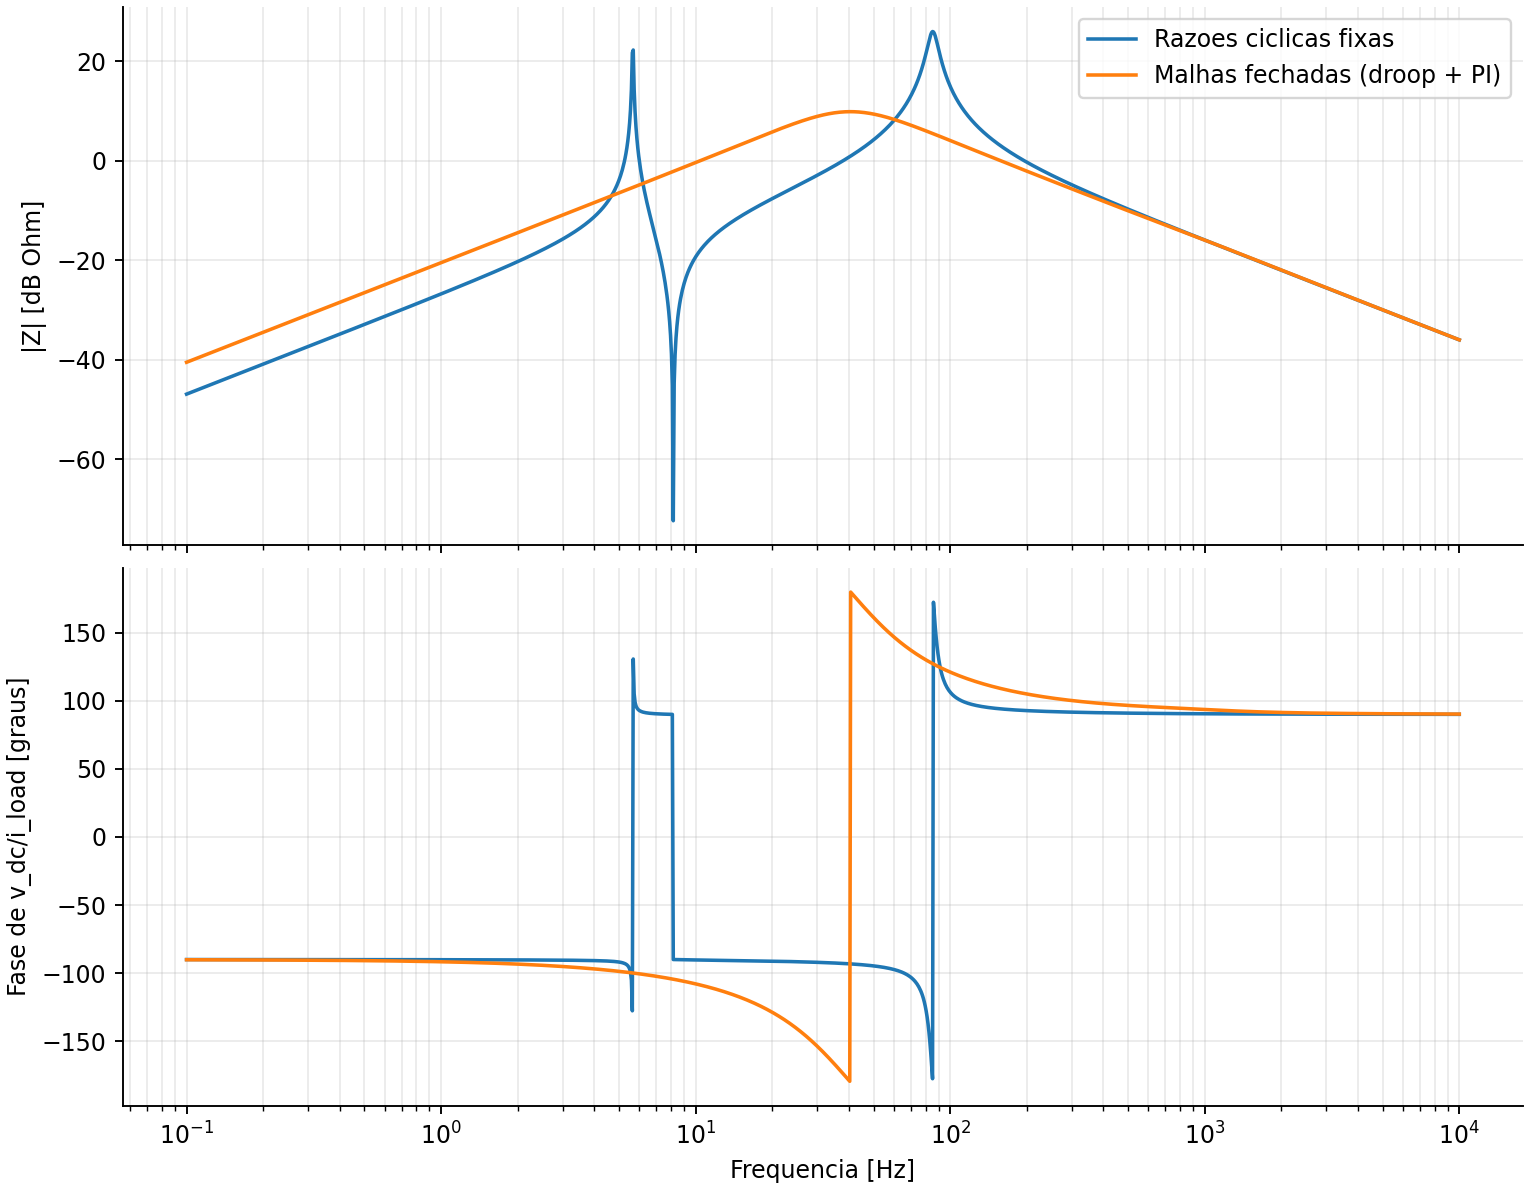
\includegraphics[width=\columnwidth]{images/fig_Z.png}
\caption{Módulo e fase de $Z_{out}$ com razões cíclicas fixas e com PI--\textit{droop}.}
\label{fig:Z}
\end{figure}

\begin{table}[H]
\centering
\caption{$|Z_{out}|$ em malha aberta (razões cíclicas fixas) e em malha fechada}
\label{tab:Z}
\small
\begin{tabular}{rcc}
\toprule
$f$ [Hz] & Razões fixas [$\Omega$] & Controle [$\Omega$] \\
\midrule
1 & 0,0461 & 0,0948 \\
10 & 0,1086 & 0,9639 \\
40 & 1,0914 & 3,1272 \\
100 & 5,6309 & 1,6058 \\
1000 & 0,1603 & 0,1602 \\
\bottomrule
\end{tabular}
\end{table}

Os autovalores do sistema com razões cíclicas fixas são $-24{,}88\pm j536{,}09$, $-0{,}119\pm j35{,}59$ e $0$. Em malha fechada, com os dez estados, obtêm-se $-4415{,}6\pm j4549{,}2$, $-4442{,}2\pm j4443{,}6$ (dois pares), $-157{,}0\pm j200{,}5$, $-12{,}56$ e $0$, apresentados na Figura~\ref{fig:eig}. O autovalor nulo está associado à ausência de regulação explícita do nível de energia do ultracapacitor, pois o controle o utiliza em transitórios sem forçar $v_c$ a um único valor permanente. Os demais modos possuem parte real negativa, e os modos pouco amortecidos da malha aberta, com parte real de $-0{,}119$, passam a ter amortecimento adequado. Contudo, não é correto afirmar estabilidade assintótica de todos os estados sem uma malha adicional de recuperação do estado de carga.

\begin{figure}[H]
\centering
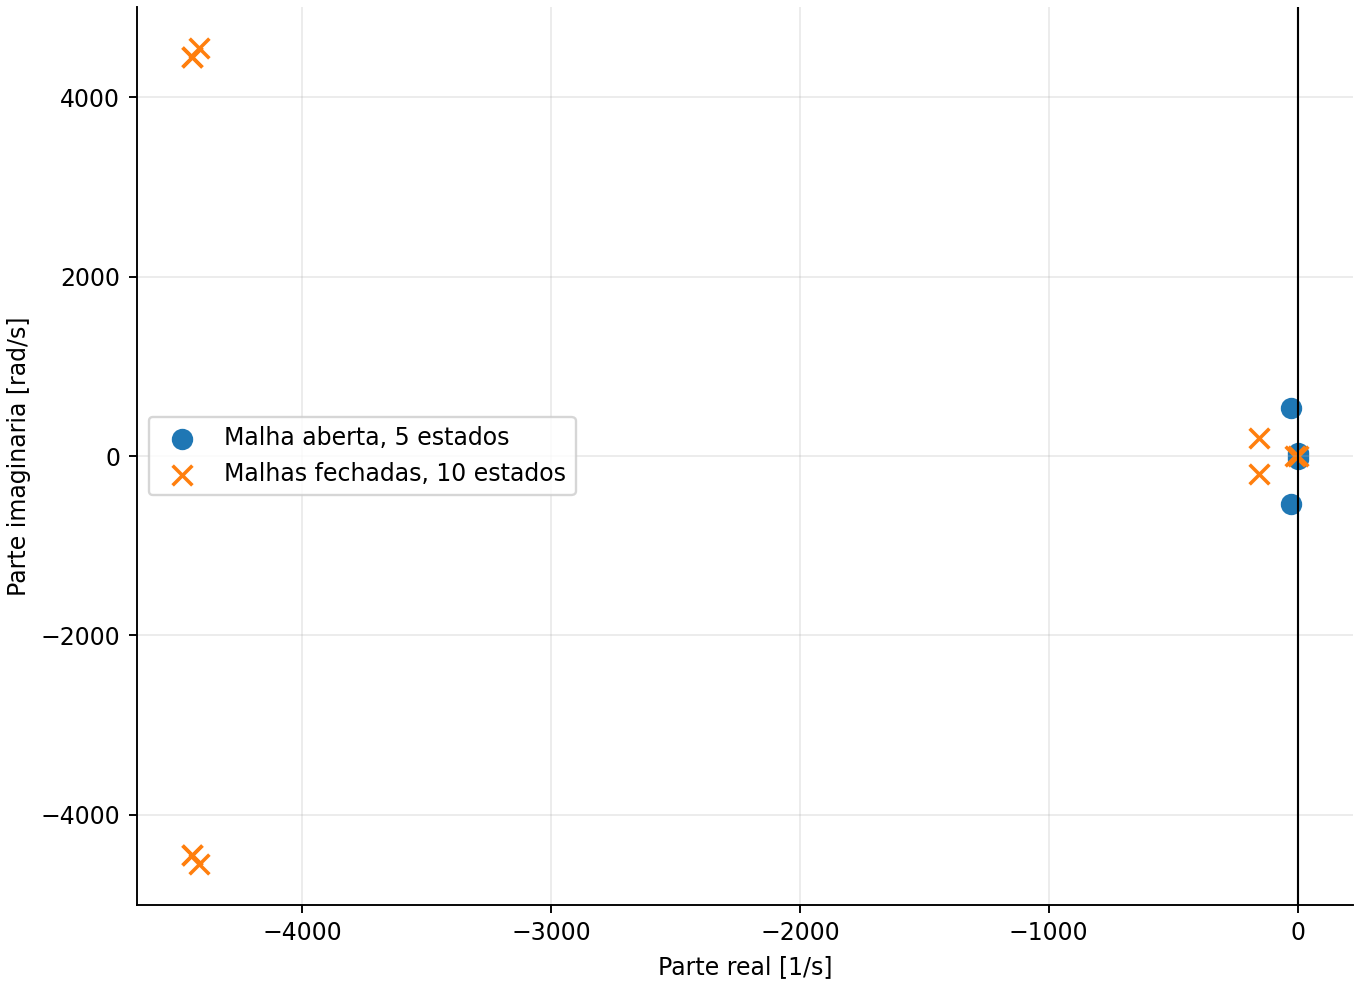
\includegraphics[width=\columnwidth]{images/fig_eig.png}
\caption{Autovalores dos modelos linearizados em malha aberta (5 estados) e fechada (10 estados).}
\label{fig:eig}
\end{figure}
